\documentclass[11pt,letterpaper]{article}

% ------------------------------------------------
% Paquetes básicos
% ------------------------------------------------
\usepackage[utf8]{inputenc}
\usepackage[T1]{fontenc}
\usepackage[spanish]{babel}
\usepackage{amsmath, amssymb}
\usepackage{graphicx}
\usepackage{booktabs}
\usepackage{float}
\usepackage{array}
\usepackage{hyperref}
\usepackage{geometry}
\usepackage{setspace}

% ------------------------------------------------
% Configuración de página
% ------------------------------------------------
\geometry{
	left=2.5cm,
	right=2.5cm,
	top=2.5cm,
	bottom=2.5cm
}

\onehalfspacing

% ------------------------------------------------
% Datos del documento
% ------------------------------------------------
\title{\textbf{Análisis de sentimientos en críticas de películas mediante modelos Transformers}}

\author{
	Sebastián Calderón Segura C21517\\
	Luis Diego Elizondo Fennell C4E844 \\
	Santiago Paniagua Chavarría C4I249\\
	Andrés Zúñiga Mora C38733\\
	\\
	Universidad de Costa Rica \\
	CA0305 - Herramientas de Ciencia de Datos II
}

\date{Julio, 2026}

\begin{document}
	
	\maketitle
	
	\begin{abstract}
		Este proyecto desarrolla una aplicación introductoria de procesamiento de lenguaje natural mediante modelos basados en Transformers. La tarea seleccionada corresponde al análisis de sentimientos en críticas de películas, donde cada texto se clasifica como positivo o negativo. Para ello, se utiliza un conjunto de datos de reseñas cinematográficas y se implementa un modelo de clasificación en Google Colab mediante Python y la librería \texttt{transformers}. Además de presentar el procedimiento computacional y los resultados obtenidos, el informe relaciona el modelo utilizado con conceptos matemáticos desarrollados en las primeras bitácoras del curso, tales como representación vectorial, matrices, probabilidades, funciones de clasificación y métricas de evaluación. Finalmente, se discute cómo este tipo de herramientas puede trasladarse a problemas actuariales relacionados con análisis de reclamos, satisfacción de clientes y riesgo reputacional.
	\end{abstract}
	
	\section{Introducción}
	
	El crecimiento de los datos no estructurados ha generado la necesidad de utilizar herramientas computacionales capaces de procesar texto de forma automática. En particular, las reseñas, comentarios y opiniones escritas contienen información subjetiva que puede ser relevante para comprender la percepción de los usuarios respecto a un producto, servicio o experiencia. Sin embargo, cuando el volumen de información es grande, el análisis manual se vuelve costoso, lento y difícil de estandarizar.
	
	A partir de esta inconveniencia, este proyecto propone utilizar un modelo basado en Transformers para realizar un análisis sobre un conjunto extenso de texto. Los modelos Transformers fueron introducidos por Vaswani et al.~\cite{vaswani2017} y se han convertido en una arquitectura central para tareas de procesamiento de lenguaje natural. En este caso, se realizará un análisis de sentimientos sobre críticas de películas.
	
	\subsection{Objetivo general}
	
	Aplicar un modelo Transformer para clasificar críticas de películas según su sentimiento, con el fin de analizar su desempeño y discutir su posible utilidad en contextos actuariales relacionados con el análisis automático de texto.
	
	\subsection{Objetivos específicos}
	
	\begin{enumerate}
		\item Seleccionar un conjunto de datos adecuado para una tarea de análisis de sentimientos.
		\item Implementar en Google Colab un modelo de clasificación de texto usando la librería \texttt{transformers}.
		\item Obtener predicciones de sentimiento para críticas de películas.
		\item Analizar los resultados mediante tablas, métricas y visualizaciones.
		\item Relacionar el funcionamiento del modelo con conceptos matemáticos desarrollados en las bitácoras anteriores.
		\item Interpretar la utilidad de este tipo de modelos en el campo actuarial.
	\end{enumerate}
	
	\subsection{Tarea seleccionada}
	
	La tarea seleccionada es análisis de sentimientos. Esta tarea pertenece al área de procesamiento de lenguaje natural y consiste en clasificar textos de acuerdo con la polaridad emocional expresada en ellos. En este caso, se trabaja con dos clases principales: sentimiento positivo y sentimiento negativo.
	
	\subsection{Justificación actuarial}
	
	Desde una perspectiva actuarial, el análisis de sentimientos puede utilizarse como una herramienta complementaria para estudiar información cualitativa proveniente de clientes o asegurados. Por ejemplo, una compañía aseguradora podría analizar comentarios sobre atención al cliente, reclamos, tiempos de respuesta o percepción del servicio. Esta información puede apoyar procesos de toma de decisiones vinculados con retención de clientes, riesgo reputacional, calidad del servicio y segmentación de usuarios.
	
	\section{Datos y análisis}
	
	\subsection{Descripción del conjunto de datos}
	
	Para el análisis se utilizó la partición \texttt{test} del conjunto de datos IMDb, disponible públicamente en Hugging Face~\cite{imdbdataset}. Esta partición contiene 25\,000 críticas de películas, cada una con una etiqueta binaria asociada al sentimiento. La etiqueta \texttt{0} representa una crítica negativa, mientras que la etiqueta \texttt{1} representa una crítica positiva. Para reducir el tiempo de ejecución en Google Colab y mantener balanceadas las clases, se seleccionó una muestra de 1000 observaciones: 500 críticas negativas y 500 críticas positivas.
	
	\begin{table}[H]
		\centering
		\caption{Distribución de sentimientos reales en la muestra}
		\label{tab:distribucion-sentimientos}
		\begin{tabular}{lrr}
			\toprule
			Sentimiento & Frecuencia & Porcentaje \\
			\midrule
			Negativo & 500 & 50\% \\
			Positivo & 500 & 50\% \\
			\bottomrule
		\end{tabular}
	\end{table}
	\subsection{Origen de los datos}
	
	Los datos fueron obtenidos del repositorio público IMDb Movie Reviews Dataset, disponible en Hugging Face~\cite{imdbdataset}. El conjunto de datos fue seleccionado porque posee una estructura clara, etiquetas definidas y una relación directa con la tarea de análisis de sentimientos. Además, su formato facilita la carga en Python y su uso con modelos disponibles en la librería \texttt{transformers}.
	
	\subsection{Preparación de los datos}
	
	El procesamiento inicial de los datos se realizó en Google Colab utilizando Python. Primero, se cargó el conjunto de datos y se transformó en un \textit{DataFrame} para facilitar su exploración. Posteriormente, se revisó la estructura de las variables, la cantidad de observaciones y la distribución de las etiquetas. Posteriormente, se seleccionó una muestra balanceada de 1000 observaciones para reducir el tiempo de ejecución del modelo.
	
	\subsection{Análisis exploratorio}
	
	Como parte del análisis exploratorio, se calculó la cantidad de críticas positivas y negativas. Este paso permite verificar si el conjunto de datos está balanceado y facilita la interpretación posterior de los resultados del modelo.
	
	\begin{table}[H]
		\centering
		\caption{Resumen descriptivo de la longitud de las críticas}
		\label{tab:longitud-criticas}
		\begin{tabular}{lrr}
			\toprule
			Estadístico & Número de palabras & Número de caracteres \\
			\midrule
			Media & 222.53 & 1258.50 \\
			Desviación estándar & 161.41 & 923.74 \\
			Mínimo & 8 & 61 \\
			Primer cuartil & 125 & 693 \\
			Mediana & 170 & 951.50 \\
			Tercer cuartil & 267 & 1509.75 \\
			Máximo & 1002 & 5765 \\
			\bottomrule
		\end{tabular}
	\end{table}
	La longitud promedio de las críticas en la muestra fue de aproximadamente 223 palabras, con una mediana de 170 palabras. Esto indica que la distribución de longitudes presenta asimetría hacia la derecha, pues existen algunas críticas considerablemente más extensas que el resto. En efecto, mientras que el 75\% de las críticas tiene 267 palabras o menos, el valor máximo observado fue de 1002 palabras. Esta variabilidad justifica el uso de un modelo de lenguaje capaz de procesar secuencias textuales de distinta longitud.
	
	Para aplicar el modelo a las críticas se utilizó procesamiento por lotes con \texttt{batch\_size=16}. Además, se aplicó truncamiento con una longitud máxima de 512 tokens, debido a que los modelos tipo BERT poseen una longitud máxima de entrada. Esta decisión permite procesar textos largos sin generar errores de ejecución, aunque implica que en críticas muy extensas solo se analiza la primera parte del texto.
	
	\section{Método y resultados}
	
	El modelo utilizado fue \texttt{distilbert-base-uncased-finetuned-sst-2-english}, disponible mediante la librería \texttt{transformers}. Este modelo corresponde a una versión reducida de BERT llamada DistilBERT, ajustada previamente para tareas de análisis de sentimientos. La implementación se realizó mediante el \textit{pipeline} \texttt{sentiment-analysis}, el cual recibe un texto como entrada y devuelve una etiqueta de sentimiento junto con un puntaje de confianza. Aunque el modelo fue ajustado originalmente sobre el conjunto SST-2, en este proyecto se evalúa su desempeño sobre IMDb, por lo que el experimento también puede interpretarse como una prueba de transferencia entre dominios.
	
	\subsection{Implementación en Google Colab}
	
	La implementación computacional se desarrolló en Google Colab. Se utilizaron principalmente las librerías \texttt{pandas}, \texttt{datasets} y \texttt{transformers}. La librería \texttt{pandas} permitió organizar los datos en forma tabular, mientras que \texttt{transformers} permitió cargar un modelo preentrenado para clasificación de sentimiento.
	
	El procedimiento general fue el siguiente:
	
	\begin{enumerate}
		\item Instalar e importar las librerías necesarias.
		\item Cargar el conjunto de datos.
		\item Convertir los datos a formato tabular.
		\item Seleccionar las variables necesarias.
		\item Aplicar el modelo Transformer a las críticas.
		\item Guardar las predicciones del modelo.
		\item Analizar los resultados obtenidos.
	\end{enumerate}
	
	\subsection{Modelo Transformer utilizado}
	
	El modelo utilizado pertenece a la familia de modelos Transformers. Estos modelos se caracterizan por transformar secuencias de texto en representaciones numéricas que capturan relaciones entre palabras y contexto. Para este proyecto, se utilizó un modelo preentrenado mediante un \textit{pipeline} de análisis de sentimientos.
	
	La salida del modelo contiene dos elementos principales:
	
	\begin{itemize}
		\item Una etiqueta de clasificación, por ejemplo, \texttt{POSITIVE} o \texttt{NEGATIVE}.
		\item Un puntaje de confianza asociado a la predicción.
	\end{itemize}
	
	\subsection{Relación matemática con las bitácoras anteriores}
	
	Una parte central del proyecto consiste en conectar el modelo utilizado con los fundamentos matemáticos y computacionales vistos en las bitácoras anteriores. Aunque el modelo se utilizó como una herramienta ya entrenada, su funcionamiento interno está compuesto en gran medida por operaciones que ya se habían estudiado en las Bitácoras 1 y 2: desde la representación del texto como tensores hasta la función de pérdida y el optimizador usados durante su entrenamiento. La siguiente tabla resume esa correspondencia.
	
	\begin{table}[H]
		\centering
		\caption{Relación entre los conceptos de las bitácoras y sus equivalentes en DistilBERT}
		\label{tab:relacion-bitacoras}
		\begin{tabular}{p{6.5cm}p{7cm}}
			\toprule
			Concepto explorado en las bitácoras & Dónde aparece dentro de DistilBERT \\
			\midrule
			Tensores, reshape, broadcasting, \texttt{einsum} (Bitácora 1) & Los embeddings de tokens y sus operaciones por lote \\
			Producto punto y \texttt{batch\_matmul} (Bitácora 1) & El cálculo de similitud Q·K\textsuperscript{T} en cada cabeza de atención \\
			Softmax estable (Bitácora 1) & Normalización de los pesos de atención y de los logits finales \\
			Cross-entropy loss (Bitácora 1) & Función de pérdida usada para el fine-tuning en SST-2 \\
			Capa lineal \texttt{linear\_forward} / \texttt{linear\_backward} (Bitácora 2) & Proyecciones Q, K, V y las capas feed-forward \\
			ReLU / sigmoid / tanh (Bitácora 2) & GELU, la no linealidad de los bloques feed-forward \\
			Layer Normalization (Bitácora 2) & Normalización después de cada bloque de atención y feed-forward \\
			Dropout (Bitácora 2) & Regularización durante el entrenamiento del modelo \\
			Xavier / Kaiming init (Bitácora 2) & Inicialización de los pesos antes de entrenar \\
			SGD, Momentum, Adam (Bitácora 2) & AdamW, el optimizador usado para ajustar los pesos \\
			\bottomrule
		\end{tabular}
	\end{table}
	
	\subsubsection{Representación vectorial del texto}
	
	Para que un modelo pueda procesar texto, las palabras deben transformarse en representaciones numéricas. Esta idea se relaciona con el uso de vectores y matrices, pues cada texto puede representarse mediante arreglos numéricos que condensan información semántica. De esta forma, un problema originalmente lingüístico se convierte en un problema matemático y computacional.
	
	\subsubsection{Matrices y transformaciones}
	
	Los modelos Transformers utilizan operaciones matriciales para transformar las representaciones de entrada. Cada capa del modelo aplica transformaciones sobre los vectores que representan las palabras o fragmentos de texto. Esta estructura se relaciona con el uso de arreglos y operaciones vectorizadas estudiadas en Python y NumPy.
	
	\subsubsection{Probabilidad y clasificación}
	
	El análisis de sentimientos puede interpretarse como un problema de clasificación. Dado un texto de entrada, el modelo asigna puntajes a las posibles clases. La clase seleccionada corresponde a aquella con mayor puntaje o probabilidad estimada. En este proyecto, las clases principales corresponden a sentimiento positivo y sentimiento negativo.
	
	\subsubsection{Métricas de evaluación}
	
	Si el conjunto de datos contiene etiquetas reales, es posible comparar las predicciones del modelo con dichas etiquetas. Algunas métricas útiles son la exactitud, la precisión, el recall y la medida F1. Estas métricas permiten evaluar qué tan bien se desempeña el modelo en la tarea de clasificación.
	
	\subsection{Resultados obtenidos}
	
	Los resultados del modelo se resumen mediante tablas y gráficos. En particular, se analiza la cantidad de críticas clasificadas como positivas y negativas, así como ejemplos específicos de predicciones realizadas por el modelo.
	
	\begin{table}[H]
		\centering
		\caption{Métricas generales del modelo}
		\label{tab:metricas-modelo}
		\begin{tabular}{lr}
			\toprule
			Métrica & Valor \\
			\midrule
			Accuracy & 0.9000 \\
			Precision & 0.9219 \\
			Recall & 0.8740 \\
			F1-score & 0.8973 \\
			\bottomrule
		\end{tabular}
	\end{table}
	
	El modelo obtuvo una exactitud global de 0.90, lo cual indica que clasificó correctamente el 90\% de las críticas de la muestra. La precisión fue de 0.9219, lo que muestra que, cuando el modelo predijo una crítica como positiva, en la mayoría de los casos dicha predicción fue correcta. El recall fue de 0.8740, por lo que el modelo identificó correctamente el 87.4\% de las críticas realmente positivas. Finalmente, el F1-score fue de 0.8973, reflejando un equilibrio adecuado entre precisión y recall.
	
	\begin{table}[H]
		\centering
		\caption{Matriz de confusión del modelo}
		\label{tab:matriz-confusion}
		\begin{tabular}{lrr}
			\toprule
			Etiqueta real / Predicción & Negativo & Positivo \\
			\midrule
			Negativo & 463 & 37 \\
			Positivo & 63 & 437 \\
			\bottomrule
		\end{tabular}
	\end{table}
	
	La matriz de confusión muestra que el modelo clasificó correctamente 463 críticas negativas y 437 críticas positivas. Sin embargo, cometió 37 errores al clasificar críticas negativas como positivas y 63 errores al clasificar críticas positivas como negativas. Esto sugiere que el modelo fue ligeramente más efectivo detectando críticas negativas que críticas positivas, lo cual también se observa en el recall por clase: 0.93 para la clase negativa y 0.87 para la clase positiva.
	
	\begin{table}[H]
		\centering
		\caption{Reporte de clasificación por clase}
		\label{tab:classification-report}
		\begin{tabular}{lrrrr}
			\toprule
			Clase & Precision & Recall & F1-score & Soporte \\
			\midrule
			Negativo & 0.88 & 0.93 & 0.90 & 500 \\
			Positivo & 0.92 & 0.87 & 0.90 & 500 \\
			\midrule
			Promedio macro & 0.90 & 0.90 & 0.90 & 1000 \\
			Promedio ponderado & 0.90 & 0.90 & 0.90 & 1000 \\
			\bottomrule
		\end{tabular}
	\end{table}
	
	También se revisaron algunos errores del modelo. En uno de los casos, una crítica etiquetada como negativa fue clasificada como positiva con una confianza de 0.9658. Este resultado muestra que una alta confianza del modelo no garantiza que la predicción sea correcta. En textos largos o ambiguos, el modelo puede enfocarse en fragmentos con aparente carga positiva y omitir el sentido general negativo de la reseña. Este comportamiento es importante porque evidencia una limitación de los modelos automáticos de lenguaje: pueden fallar ante ironía, contradicciones, ambigüedad o estructuras discursivas complejas.
	
	
	\begin{figure}[H]
		\centering
		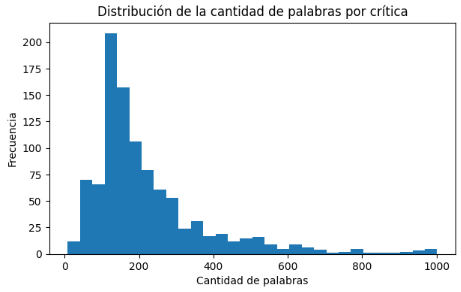
\includegraphics[width=0.75\linewidth]{graficos/cantidadcritica.png}
		\caption{Distribución de la cantidad de palabras por crítica}
		\label{fig:cantidad-palabras}
	\end{figure}
	
	La Figura~\ref{fig:cantidad-palabras} presenta la distribución de la cantidad de palabras por crítica. Se observa que la mayoría de las críticas se concentra entre aproximadamente 100 y 300 palabras, aunque existen textos considerablemente más largos. Esta variabilidad en la longitud de los textos justifica el uso de un modelo de lenguaje capaz de procesar secuencias textuales de distinta extensión.
	
	\begin{figure}[H]
		\centering
		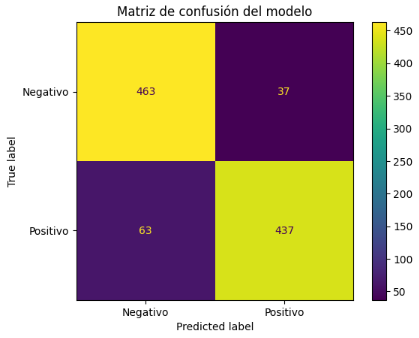
\includegraphics[width=0.65\linewidth]{graficos/matrizconfusion.png}
		\caption{Matriz de confusión del modelo Transformer}
		\label{fig:matriz-confusion}
	\end{figure}
	
	La Figura~\ref{fig:matriz-confusion} resume el desempeño del modelo sobre la muestra evaluada. El modelo clasificó correctamente 463 críticas negativas y 437 críticas positivas. Además, clasificó erróneamente 37 críticas negativas como positivas y 63 críticas positivas como negativas. En conjunto, estos resultados muestran un desempeño general favorable, aunque también evidencian que el modelo presenta errores en textos ambiguos o con estructuras discursivas complejas.
	
	\section{Conclusiones}
	
	El proyecto logró demostrar la efectividad de los modelos basados en Transformers para el análisis de sentimientos en críticas de películas. El modelo DistilBERT alcanzó una exactitud del 90\%, con métricas de precisión, recall y F1-score cercanas al 0.90, lo que evidencia un desempeño sólido y balanceado en la clasificación de textos positivos y negativos.
	
	Desde el punto de vista actuarial, este tipo de herramientas representa una oportunidad para incorporar información no estructurada en procesos de análisis. En particular, los modelos de lenguaje pueden apoyar el estudio de reclamos, comentarios de clientes, encuestas de satisfacción y riesgo reputacional. Sin embargo, también es importante reconocer que el uso de un dataset de películas no representa directamente un contexto asegurador, por lo que una aplicación profesional requeriría datos específicos del sector.
	
	\subsection{Limitaciones}
	
	\begin{itemize}
		\item El conjunto de datos pertenece al contexto cinematográfico y no al sector asegurador.
		\item El modelo puede presentar dificultades ante textos irónicos, ambiguos o con sarcasmo.
		\item Si se utiliza una muestra reducida, los resultados pueden no representar completamente el conjunto de datos original.
		\item La clasificación binaria limita el análisis a sentimientos positivos y negativos, dejando por fuera categorías neutrales o mixtas.
	\end{itemize}
	
	\subsection{Aplicaciones futuras}
	
	Como extensión del proyecto, se podría utilizar un conjunto de datos relacionado directamente con aseguradoras, reclamos o comentarios de clientes. También sería posible ajustar un modelo específico para el contexto actuarial, incorporar una categoría neutral o combinar el análisis de sentimientos con variables cuantitativas.
	
	\section{Disponibilidad de código y datos}
	
	El desarrollo computacional fue realizado en Google Colab. El código, los datos procesados, los resultados y los gráficos se encuentran disponibles en el repositorio del grupo y en el Google Colab:
	
	\begin{center}
		\href{https://github.com/JavaLuisdi/CA0305---Proyecto-grupal}{Repositorio del proyecto en GitHub}
		\quad
		\href{https://colab.research.google.com/drive/1K8V-G299sKaaA0yxnt4jAEjhzKXfEFx8?usp=sharing#scrollTo=JKRvCUxRTkJs}{Google Colab}
	\end{center}
	
	%\section*{Referencias}
	
	\begin{thebibliography}{9}
		
		\bibitem{vaswani2017}
		Vaswani, A., Shazeer, N., Parmar, N., Uszkoreit, J., Jones, L., Gomez, A. N., Kaiser, L., \& Polosukhin, I. (2017). Attention is all you need. \textit{Advances in Neural Information Processing Systems}.
		
		\bibitem{mckinney2022}
		McKinney, W. (2022). \textit{Python for Data Analysis}. O'Reilly Media.
		
		\bibitem{huggingface2024}
		Hugging Face. (2024). \textit{Transformers documentation}. \url{https://huggingface.co/docs/transformers}
		
		\bibitem{imdbdataset}
		Stanford AI Lab. (2024). \textit{IMDb Movie Reviews Dataset}. \url{https://huggingface.co/datasets/stanfordnlp/imdb}
		
	\end{thebibliography}
	
\end{document}